\section{Affinity Graph and Batch Structure}
\label{app:graph_structure}

The affinity graph $P$ is computed using an adaptive Gaussian (RBF) kernel in PCA space, following the SEACells protocol~\citep{seacells} with default hyperparameter choices (15 nearest neighbors for bandwidth estimation).
Because PCA embeddings reflect both biological variation and technical batch effects, the resulting graph encodes a mixture of biological and batch-driven proximity.
Figure~\ref{fig:graph_umap} visualizes this directly: a UMAP embedding of the affinity matrix on the Pancreas dataset~\citep{luecken2020benchmarking} reveals clear batch structure alongside biological cell-type organization.
This confirms that the input graph is not batch-free, and motivates the batch-conditional encoder design, which explicitly disentangles these signals during training rather than requiring a pre-corrected graph.

\begin{figure}[h]
\centering
% TODO: insert figure -- UMAP computed from the RBF affinity matrix on the Pancreas dataset,
% colored by (left) batch label and (right) cell type.
% In scanpy: set adata.obsp['connectivities'] = P, then sc.tl.umap(adata).
\includegraphics[width=\textwidth]{figures/pancreas_aff.png}
\caption{
UMAP of the precomputed RBF affinity graph on the Pancreas dataset.
Left: colored by cell type. Right: colored by batch label.
Batch structure is clearly visible in the graph embedding, confirming that the input affinity graph reflects both biological and technical variation.
The batch-conditional encoder disentangles these signals during training.
}
\label{fig:graph_umap}
\end{figure}


\section{Training Details and Hyperparameters}
\label{app:training}

\paragraph{Architecture.}
The encoder and decoder follow the scPoli architecture~\citep{scpoli} with default settings: hidden dimension 64, latent dimension 8, and 50 PCA components as input features.

\paragraph{Optimizer.}
We use Adam~\citep{adam} with learning rate $3 \times 10^{-4}$, $\varepsilon = 0.01$, and weight decay $10^{-5}$.
Batch embedding parameters are excluded from weight decay to avoid penalizing dataset-specific offsets.
A linear warmup over 5 epochs is followed by cosine learning rate decay.

\paragraph{Batch size.}
Mini-batches contain 1024 cells sampled uniformly across batches.

\paragraph{Training stages.}
Stage 1 (CVAE pretraining) runs for 25 epochs.
Stage 2 (joint prototype learning) uses early stopping based on modularity, evaluated every few epochs, with a minimum improvement threshold of 0.005 and 1000 gradient steps per epoch.

\paragraph{Loss weights.}
The total objective is
\[
\mathcal{L} = \mathcal{L}_{\text{community}} + \lambda\,\mathcal{L}_{\text{rec}} + \lambda_n\,\mathcal{L}_{\text{nassoc}} + \lambda_u\,\mathcal{L}_{\text{usage}},
\]
with $\lambda = 0.01$, $\lambda_n = 1.0$, and $\lambda_u = 0.1$.
The normalized association loss uses element-wise max aggregation across batches ($\alpha = 1.0$).
These values were chosen to balance community structure preservation against reconstruction fidelity, and were not tuned per dataset.

\paragraph{Gradient flow in $\mathcal{L}_{\text{rec}}$.}
Although the soft assignments $s_{ik}$ depend on the encoder output $z_i$, we stop the gradient through $s_{ik}$ when backpropagating $\mathcal{L}_{\text{rec}}$.
Reconstruction gradients therefore reach only the decoder $g_\phi$ and the prototype vectors $\{c_k\}$ (via their role as decoder inputs); the encoder $f_\theta$ receives no gradient from $\mathcal{L}_{\text{rec}}$.
The motivation is to keep the two objectives from pulling the encoder in conflicting directions: $\mathcal{L}_{\text{community}}$ encourages encoder outputs to reflect affinity-graph structure, while an unconstrained $\mathcal{L}_{\text{rec}}$ gradient could push the encoder toward assignments that minimise reconstruction error regardless of graph proximity.
By stopping the gradient, the encoder is shaped exclusively by $\mathcal{L}_{\text{community}}$, while the prototypes are jointly regularised by both objectives: they must sit at the centre of well-connected cell communities \emph{and} be decodable to meaningful gene-expression profiles.

\paragraph{Number of prototypes $K$.}
Following SEACells~\citep{seacells}, we set $K = \lceil N / 75 \rceil$, where $N$ is the total number of cells.
This yields approximately one metacell per 75 cells and provides a natural starting point for unannotated datasets.
The ratio of 75 cells per metacell reflects a target aggregation granularity that preserves rare populations while achieving meaningful compression.
Users may increase $K$ for finer resolution or decrease it for coarser summaries.

\paragraph{Graph construction.}
The affinity graph uses an adaptive Gaussian (RBF) kernel in 50-dimensional PCA space, with 15 nearest neighbors used to estimate per-cell bandwidth, following the SEACells protocol~\citep{seacells}.
All graph hyperparameters are kept at their SEACells defaults across all experiments.

For spatial experiments, the affinity is computed on spatially aggregated features rather than individual cell PCA embeddings.
Specifically, for each cell $i$, we identify all cells within a fixed spatial radius $r$ (in physical coordinates), and compute the average of their PCA embeddings as the cell's contextual feature vector.
The same adaptive Gaussian kernel is then applied to these aggregated features to construct the affinity graph.
This encodes microenvironmental context into the affinity: cells embedded in similar spatial neighborhoods---regardless of their individual transcriptomic state---are encouraged to share prototype assignments.

Figure~\ref{fig:spatial_graph_umap} visualizes the resulting affinity on the NSCLC dataset~\citep{pentimalli2025combining}: a UMAP of the spatial affinity matrix reveals that the graph captures both niche structure and cell-type organization, confirming that spatially aggregated features encode microenvironmental context beyond individual transcriptomic identity.

\begin{figure}[h]
\centering
\includegraphics[width=\textwidth]{figures/spatial_graph_umap}
\caption{
UMAP of the precomputed spatial affinity graph on the NSCLC dataset.
Left: colored by cell type. Right: colored by niche label.
The affinity captures both cell-type identity and niche-level spatial organization, motivating its use as an alternative similarity signal for metacell construction.
}
\label{fig:spatial_graph_umap}
\end{figure}

\section{Temperature Calibration}
\label{app:calibration}

The temperature $\tau$ in the soft assignment formula controls the sharpness of prototype assignments: a smaller $\tau$ yields near-one-hot assignments concentrated on a single prototype, while a larger $\tau$ spreads probability across many prototypes. Rather than setting $\tau$ as a fixed hyperparameter, we calibrate it from data after encoder pretraining and prototype initialization.

\paragraph{Effective number of prototypes.}
We characterize assignment sharpness through the effective number of prototypes per cell,
\[
\mathrm{effk}_i = \frac{1}{\displaystyle\sum_{k} s_{ik}^2},
\]
which equals 1 when a cell is assigned entirely to one prototype and $K$ when assignments are perfectly uniform.

\paragraph{Default calibration: affinity-matching.}
For dot-product similarity ($q_{ij} = s_i^\top s_j$), we calibrate $\tau$ so that the expected assignment similarity on positive edges matches the expected affinity weight:
\[
\mathbb{E}_{(i,j) \sim P}\bigl[s_i^\top s_j\bigr] = \mathbb{E}_{(i,j) \sim P}\bigl[P_{ij}\bigr].
\]
Intuitively, this sets the temperature so that the degree of overlap between prototype assignments on truly connected cell pairs mirrors the strength of their affinity. We solve for $\tau$ via binary search, holding the encoder logits fixed.

If the target is unreachable (i.e., even at the sharpest feasible $\tau$ the left-hand side cannot reach the right-hand side), or if the resulting mean effective number of prototypes falls below 3 (indicating over-collapse), we fall back to effective-$k$ alignment.

\paragraph{Fallback: effective-$k$ alignment.}
We binary-search for $\tau$ such that the mean effective number of prototypes per cell equals a target $K_\mathrm{eff}$:
\[
\mathrm{mean}_i\,\mathrm{effk}_i = K_\mathrm{eff}.
\]
The target $K_\mathrm{eff}$ is derived from the median effective number of neighbors in the affinity graph, $\mathrm{effk}_i^{\mathrm{aff}} = 1/\sum_j P_{ij}^2$. This alignment ensures that assignment sharpness is commensurate with the local neighborhood structure of the data. This fallback is also the default for non-dot-product similarity metrics, for which the affinity-matching criterion is not meaningful.

Calibration runs once on the full dataset immediately after prototype initialization and before joint optimization begins.

\section{Additional Results}
\label{app:results}

\begin{figure*}[h]
\centering
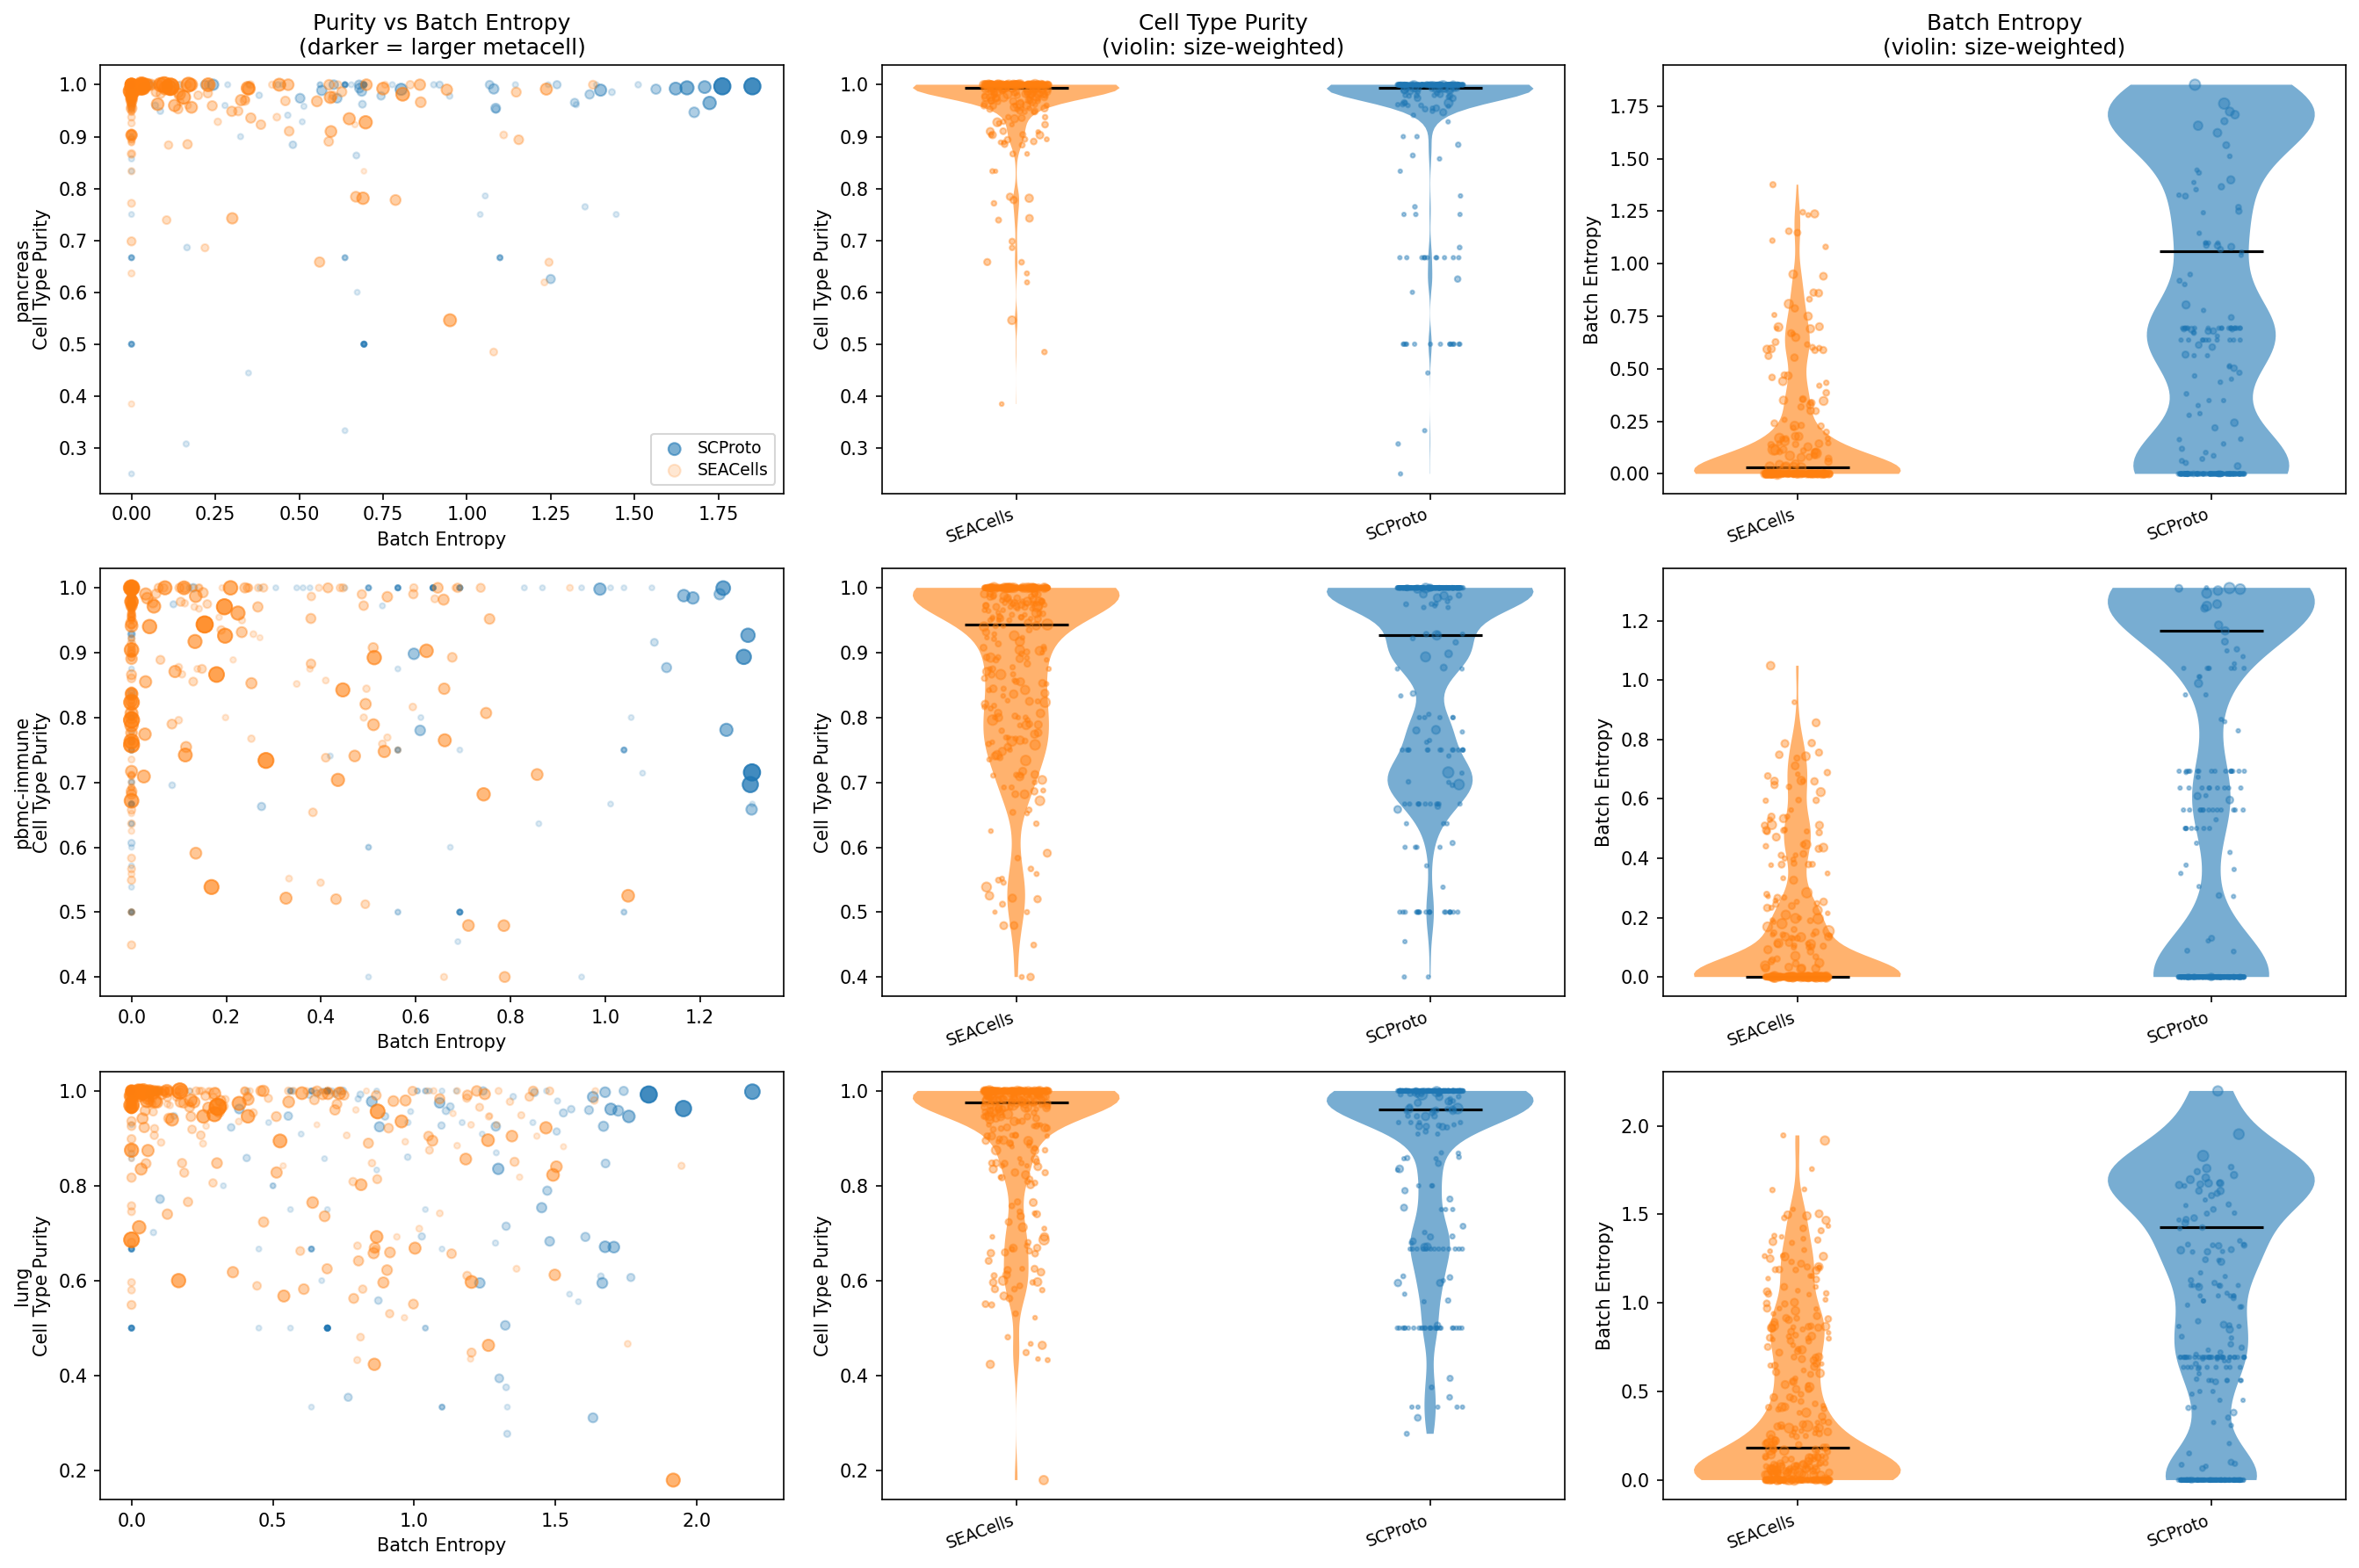
\includegraphics[width=\textwidth]{figures/pancreas_fig1.png}
\caption{
Per-metacell analysis of purity and batch mixing on the Pancreas dataset.
Left: Cell-type purity vs. batch entropy (point size proportional to metacell size).
Middle: Distribution of cell-type purity (size-weighted violin).
Right: Distribution of batch entropy (size-weighted violin).
scProto achieves higher batch entropy while maintaining comparable purity to SEACells.
}
\label{fig:purity_entropy}
\end{figure*}

\begin{figure*}[h]
\centering
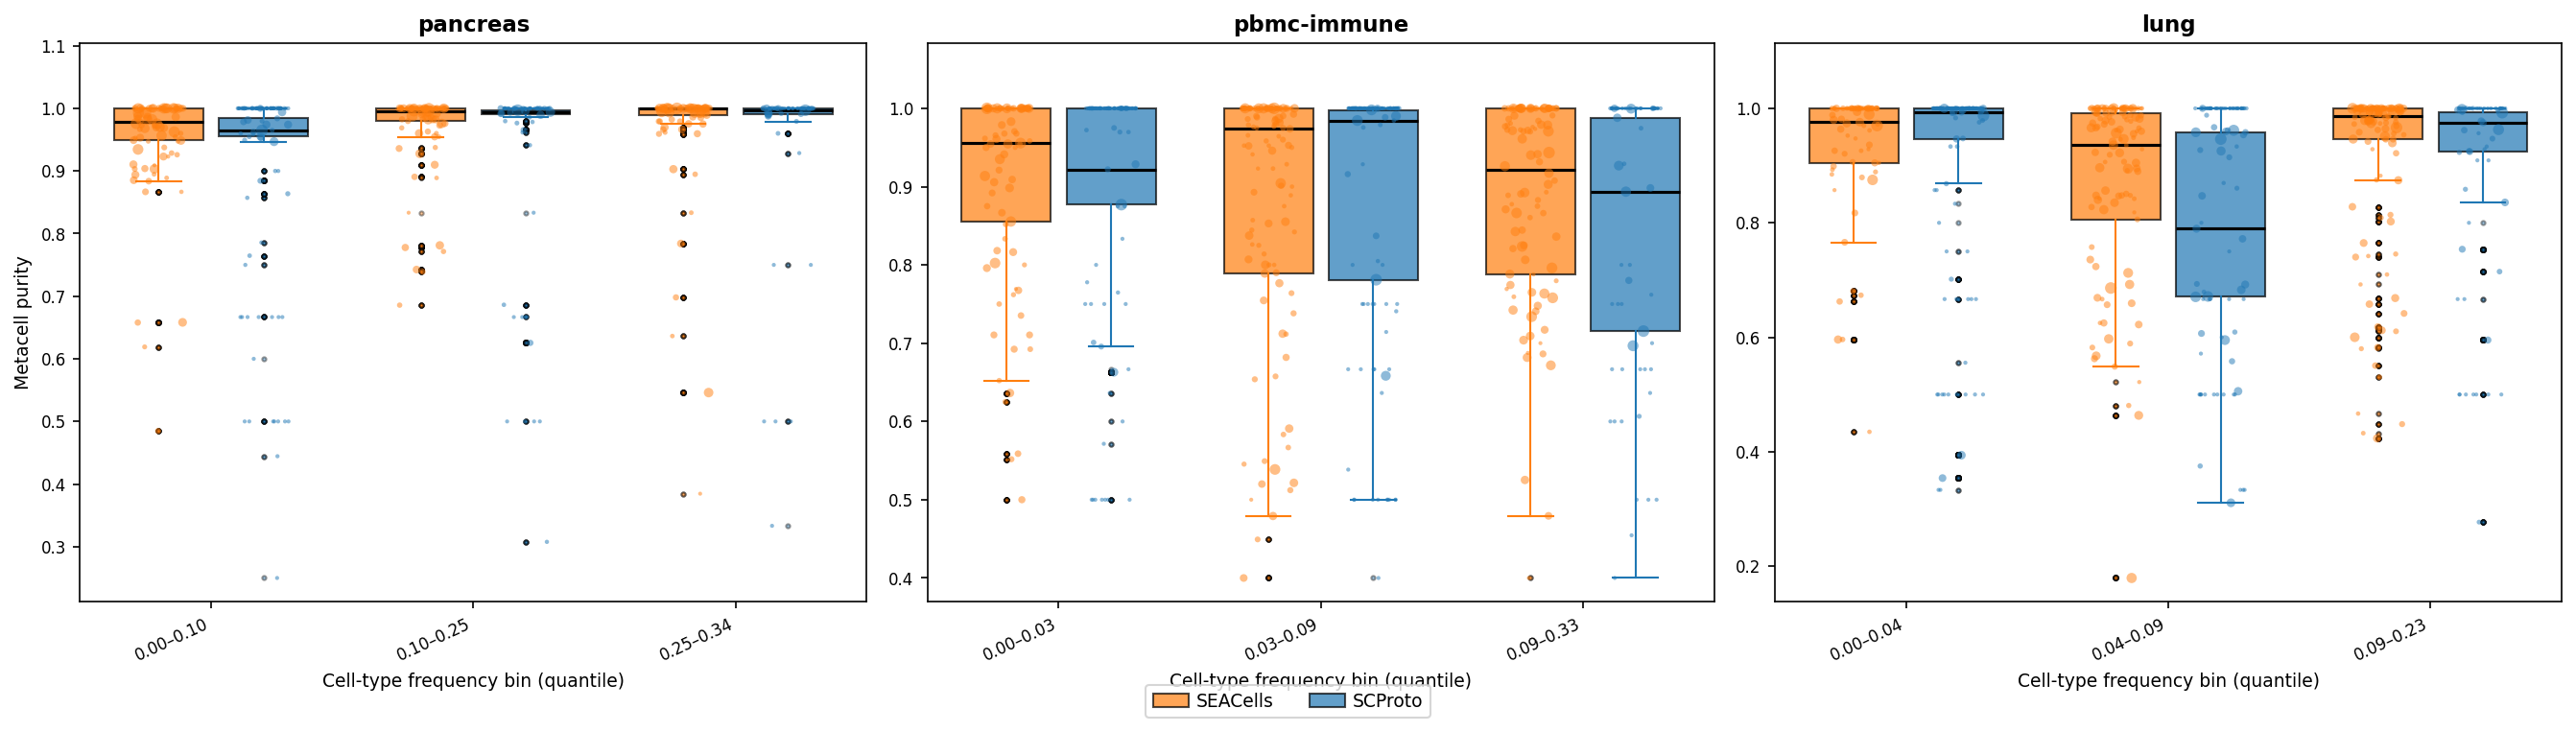
\includegraphics[width=\textwidth]{figures/freq_purities.png}
\caption{
Metacell purity stratified by cell-type frequency.
Cell types are grouped into frequency bins (quantiles), with lower-frequency bins corresponding to rare cell types.
Each point represents a metacell, and boxplots summarize the distribution.
scProto maintains high purity across all frequency bins, while SEACells shows a clear degradation in purity for rare cell types.
}
\label{fig:rare_purity}
\end{figure*}

\begin{figure*}[h]
\centering
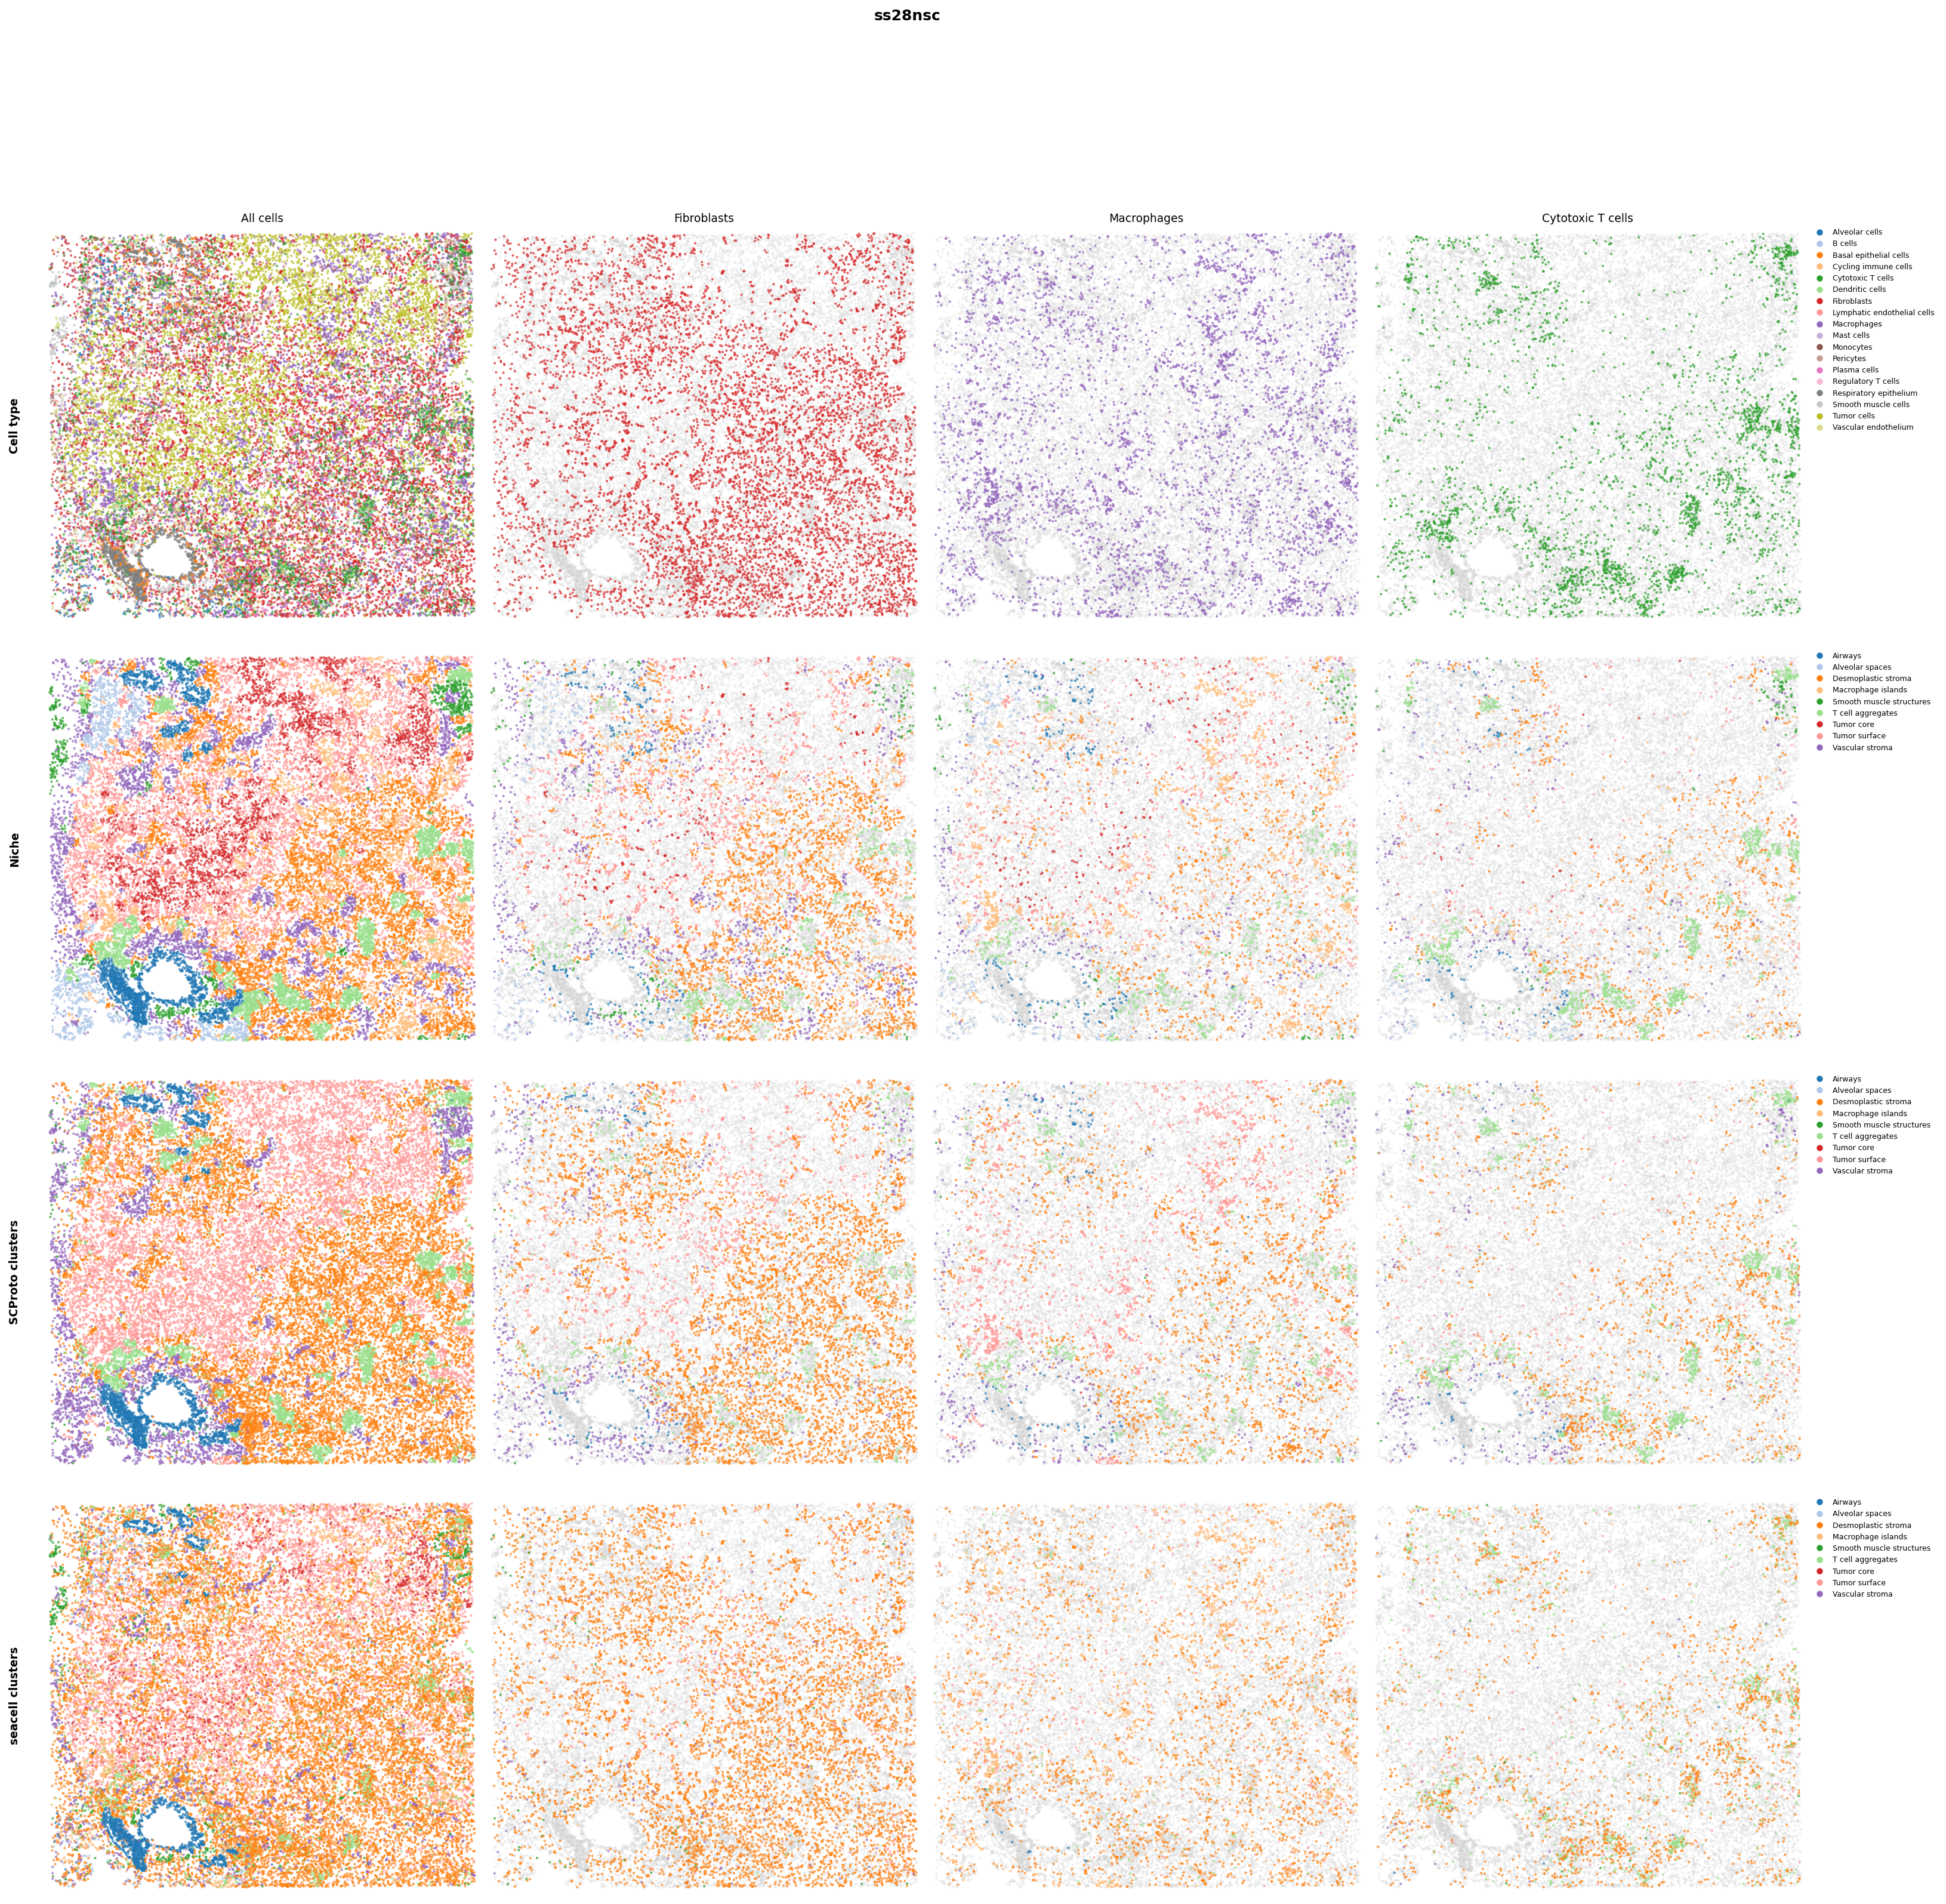
\includegraphics[width=\textwidth]{figures/spatial.png}
\caption{
Spatial visualization of cell types, niches, and metacell assignments across methods.
Columns correspond to selected cell types (fibroblasts, macrophages, cytotoxic T cells), and rows show cell-type annotations, niche annotations, scProto metacells (trained on spatial affinity), and SEACells metacells (trained on the same affinity).
In the annotation rows, each cell is colored by its ground-truth niche label; in the metacell rows, each cell is colored by the majority niche label of its assigned metacell.
scProto produces spatially coherent patterns aligned with niche structure, while SEACells exhibits more fragmented patterns.
}
\label{fig:spatial}
\end{figure*}

